\documentclass[11pt]{scrartcl}
\usepackage{graphicx}
\graphicspath{{./}}
\usepackage[sexy]{evan}
\usepackage[normalem]{ulem}
\usepackage{hyperref}
\usepackage{mathtools}
\hypersetup{
    colorlinks=true,
    linkcolor=blue,
    filecolor=magenta,      
    urlcolor=cyan,
    pdfpagemode=FullScreen,
    }
\usepackage[most]{tcolorbox}
\renewcommand{\dangle}{\measuredangle}

\renewcommand{\baselinestretch}{1.5}

\addtolength{\oddsidemargin}{-0.4in}
\addtolength{\evensidemargin}{-0.4in}
\addtolength{\textwidth}{0.8in}
% \addtolength{\topmargin}{-0.2in}
% \addtolength{\textheight}{1in} 


\setlength{\parindent}{0pt}

\usepackage{pgfplots}
\pgfplotsset{compat=1.15}
\usepackage{mathrsfs}
\usetikzlibrary{arrows}

\title{Session 1 - Warm Up}
\author{Azzam Labib (IG: haxuv.world)}
\date{G3-4 | \today}
\begin{document}
\maketitle

\begin{enumerate}
    \item There are 4 red marbles, 6 yellow marbles and 5 blue marbles in a bag. How many marbles should be picked up randomly to ensure 2 blue marbles are picked?
    
    \vspace{10cm}\item Patrick paid \$105 for buying 4 cup noodles and 7 bottles of juice. Given that the cost of each cup noodle is 2 times of the cost of each bottle of juice. How many dollars is the price of each cup noodle?

    \vspace{10cm}\item Find the value of the following expression.
    \[2024 \div 9 - 2018 \div 5 - 2006 \div 9 + 2023 \div 5\]
    
    \vspace{10cm}\item Given $1001 = 7 \times 11 \times 13$, find the sum of the three greatest factors of $214214$.

    \newpage
    \vspace{10cm}\item Given that both the length and the width of a rectangle are integers in centimetres. And the perimeter of the rectangle is 170 centimetres. How many square centimetres is the maximum area of the rectangle?
    
    \vspace{10cm}\item Find the units digit of the result of the following expression.
    \[3 \times 6 \times 9 \times \dots \times 2019 \times 2022 \times 2024\]
    
    \vspace{10cm}\item Find the value of the following expression.
    \[\frac{1}{2024} + \frac{2}{2024} + \frac{3}{2024} + \cdots + \frac{86}{2024} + \frac{87}{88} + \frac{89}{2024}\]

    \vspace{10cm}\item There is a big lake with perimeter of 400 metres. Patrick, who lives beside the lake, wanted to plant trees around the lake. On the first day, starting from his home, he planted an apple tree every 4 metres. On the second day, starting from his home, he planted an orange tree every 10 metres if there is no apple trees at that position. How many trees has he planted in total?
    
    \vspace{10cm}\item In the figure, a large rectangle is formed by 5 identical small rectangles. Given that the area of the large rectangle is 1470 square meters, how many meters is the perimeter of a small rectangle?
    \begin{figure}[h]
        \centering
        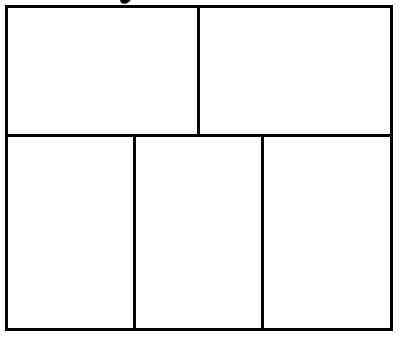
\includegraphics{StarGen/AIMO Trial G3-4 2024/5rect.png}
    \end{figure}
    
    \vspace{10cm}\item If the nine-digit number $2024A323A$ is divisible by 9, find the value of $A$.
    
    \vspace{10cm}\item Oliver has some 1 cent coins, 2 cent coins and 5 cent coins. Given that the number of 1 cent coins is 14 times of that of 2 cent coins, and the total value of the coins is 120 cents. Find the number of 5 cent coins.

    \vspace{10cm}\item Given that both the base and the height of a triangle are integers in centimetres and the area of the triangle is 219 square centimetres. How many possible combination(s) of the base and the height is / are there?
    
    \vspace{10cm}\item Find the value of the following expression.
    \[101^2 - 98^2 + 95^2 - 92^2 + 89^2 - \cdots - 11^2 + 8^2 - 5^2 + 2^2\]
    
    \vspace{10cm}\item Amy, Bella, Chris and Debby have 200 candies in total. Amy gave Bella 13 candies. Then Chris gave Debby 20 candies. Then Bella gave Chris half of all her candies. Finally Debby gave Amy 24 candies. Then they have the same number of candies. How many candies did Bella originally have?
    
    \vspace{10cm}\item Four friends have some golden coins. Nala and Freya have 32 coins together. Freya and Gracie have 46 coins together. Gracie and Greesel have 45 coins together. How many coins do Nala and Greesel have together?
    
    \vspace{10cm}\item Among the 2024 natural numbers from 1 to 2024, at least how many numbers need to be picked such that there must be two numbers having a difference of 103?
    
    \vspace{10cm}\item A dormitory is allocating the rooms. If there are 6 students living in each room, there will be 12 students not having rooms; if there are 8 students living in each room, there will be exactly 5 vacant rooms. How many students are there?

    \vspace{10cm}\item Define the operation symbol $\oplus$ following this pattern:
    \begin{align*}
        1 \oplus 5 &= 1 + 2 + 3 + 4 - 5\\
        3 \oplus 8 &= 3 + 4 + 5 + 6 + 7 - 8\\
        5 \oplus 9 &= 5 + 6 + 7 + 8 - 9\\
        \dots& \text{(and so on ...)}
    \end{align*}
    Find the value of $(5 \oplus 10) - (4 \oplus 9).$
    
    \vspace{10cm} \item How many rectangles are there in this figure?
    \begin{figure}[h]
        \centering
        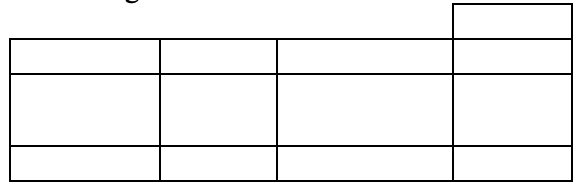
\includegraphics{StarGen/AIMO Trial G3-4 2024/howmanyrect.png}
    \end{figure}
    
    \vspace{10cm}\item There are 5 numbers, in which two of them are equal. After summing up 4 of these numbers in different ways, 4 sums are found: 163, 164, 165 and 166. Which one of these five numbers appeared twice?
\end{enumerate}

\end{document}